\begin{problem}
  Construct a program to calculate the best $L_1$ approximation in
  $\mathcal{P}_1$ to the data
  
  \begin{table}[!ht]
    \caption{Data to be approximated}
    \label{tab:data}
    \begin{center}
      \begin{tabular}{| c | c  c c c c c c | }
        \hline			
        $x_i$ & 0 & 1 & 2 & 3 &4 & 5 & 6 \\
        \hline
        $f(x_i)$ & -35 & -56 & 0 & -16 & -3 & 4 & 10 \\
        \hline  
      \end{tabular}
    \end{center}
  \end{table}
  Take all weights equal to one. Plot your approximation together with the data.
\end{problem}


\begin{solution}
  In this task, theorem 15.3 is our best friend. The theorem states
  the existence of a best approximation such that an element of
  $\mathcal{A}$ that is zero in all the points the error is zero will
  be identically equal to zero. Theorem 15.3 tells us that the a best
  approximation will go through two of the points. There is only a
  finite number of points and each pair of points have a unique
  polynomial $p \in \mathcal{P}_1$ shown in
  equation~\ref{eq:interpolation} that interpolates $f$ in those
  point.
  
  \begin{equation}
    \label{eq:interpolation}
    p(x) = \frac{f(x_j)x_i - f(x_i) x_j}{x_i - x_j} + 
    \frac{f(x_i) - f(x_j)}{x_i - x_j} \times x
  \end{equation}

  Our algorithm test every combination of points to interpolate with
  and finds the one with the smallest $\mathcal{L}_1$ error. The
  resulting polynomial is shown in equation~\ref{eq:5:approx}. The
  approximating data points in table~\ref{tab:approx}. Finally a plot
  of the approximation function with the data can be found in
  figure~\ref{fig:task_5}.
  
  \begin{equation}
    \label{eq:5:approx}
    p^*(x) =  7.8*x + -35.0
  \end{equation}
  
  \begin{table}[!ht]
    \caption{Approximation data compared to the actual}
    \label{tab:approx}
    \begin{center}
      \begin{tabular}{| c | c  c c c c c c | }
        \hline			
         $p^*(x_i)$ & -35 & -27 & -19 & -12 &-3.8 & 4 & 11 \\
        \hline
        $f(x_i)$ & -35 & -56 & 0 & -16 & -3 & 4 & 10 \\
        \hline  
      \end{tabular}
    \end{center}
  \end{table}


  \begin{figure}[!ht]
    \centering
    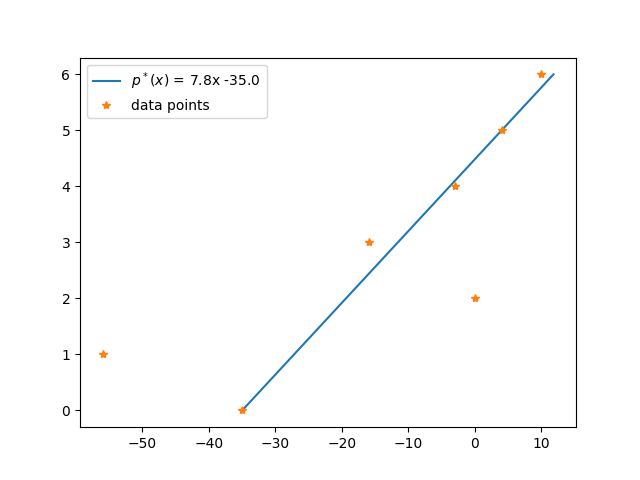
\includegraphics[scale = 0.5]{code/task_5.png}
    \caption{The data in~\ref{tab:data} together with the best
      approximation.}
    \label{fig:task_5}
  \end{figure}

\end{solution}


%%% Local Variables:
%%% mode: latex
%%% TeX-master: "report"
%%% End:
